\documentclass[a4paper,10pt]{article}
\usepackage[utf8]{inputenc}

% increase margins
\usepackage{fullpage}
\usepackage[left=1in,top=1in,right=1in,bottom=1in,headheight=3ex,headsep=3ex]{geometry}

% this puts two lines between paragraphs and no indent
\usepackage[parfill]{parskip}

% set up colors
\usepackage{array, xcolor}
\usepackage{color,hyperref}
\usepackage{graphicx}

\definecolor{torontoblue}{HTML}{00204E}
\definecolor{linkblue}{HTML}{0000FF}

% define hyperlink style
\hypersetup{colorlinks,breaklinks,
            linkcolor=linkblue,urlcolor=linkblue,
            anchorcolor=linkblue,citecolor=linkblue}

%opening
\title{Weekly Journal}
\author{Leila Uy}



\begin{document}

\maketitle

%this is commented out, no need for abstract in  your weekly assignment
% \begin{abstract}
% 
% \end{abstract}

\section{Work Update}

For this past week, I focused on creating a structure for my parallel K-means clustering algorithm. 
When reviewing the base code, Jishnu and I saw that you used \verb|kmeans| which is the part we are most 
focused on adding upon. I am thinking that we wil not be using that function because we want to experiment 
with different forms of optimization.

\subsection{Speed Testing}
Last week, I said that I wanted to test the code for this week but I had a realization that different processors 
will result in different times. My laptop has an Intel Core i7-7560U CPU with clock speed of 2.40GHz which is 
different than the processors offered by AWS  which include Intel Xeon, AMD EPYC, and AWS Graviton. Therefore, 
for more consistent timing, I should do speed testing later.

\subsection{Flowchart}
\begin{figure}[h!]
    \caption{Flowchart of the parallel K-means clustering algorithm that I want to create}
    \centering
    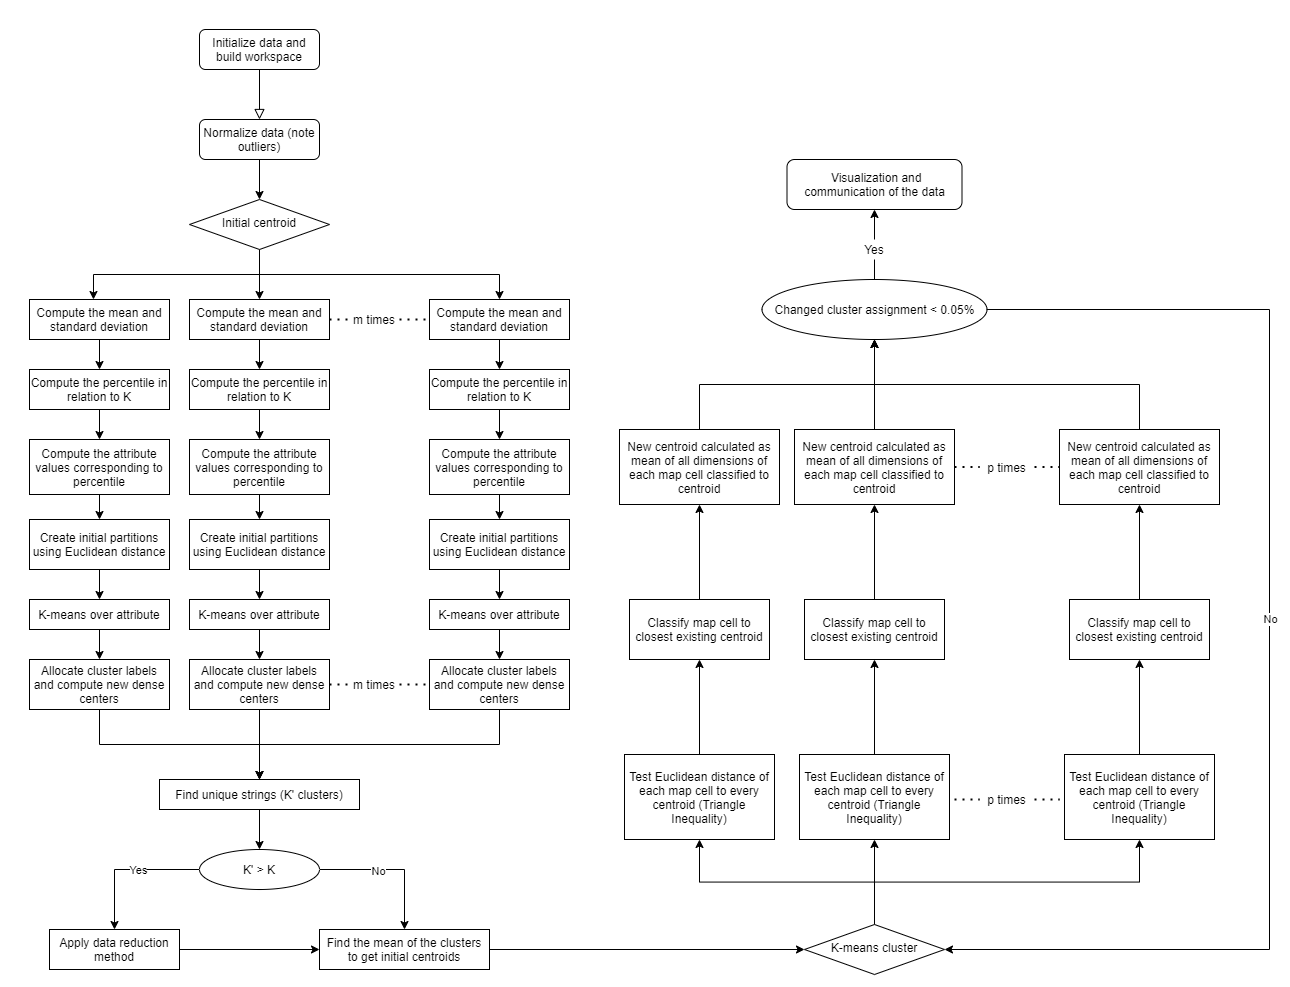
\includegraphics[scale=0.34]{flowchart.png}
\end{figure}

\section{Literature Review}
\subsection{Initial centroid}
The performance of iterative clustering algorithms like k-means clustering depend on initial cluster centroids. 
The more clusters there are, the more possibility that the random initial cluster centroids fail to find all 
the clusters correctly or lead to poor optimization. 

Several studies in the past have determined several algorithms in creating more accurate initial centorids. 
Jishnu referred me to a paper that based their algorithm on the observation that patterns can be very similar to 
each other and attributes will provide information about initial cluster centers \cite{khan2004cluster}. I 
incorporated this algorithm into my flowchart but I am open to other algorithms to finding initial centroids.

A 2020 research paper did a comparison between three hybrid methods of k-means clustering (genetic, MST, and 
hierarchical) \cite{pourahmad2020does}. They found that there was no significant improvement between the hybrid 
methods and the ordinary k-means algorithm and in some cases had poorer performance. Previous studies reported 
better performance, so the article encouraged more simulation, but it is good to note that my algorithm could 
worsen our performance and not show a significant difference in clusters. Therefore, it would be good to 
experiment with different algorithms.

In the beginning, I will initially use random selection for my initial centroids and focus on the optimization 
of the k-means clustering algorithm through parallelization and triangular inequality similar to the article we 
read first week \cite{kumar2011parallel}. Once I complete the rest of my K-means clustering in parallel, I want 
to go back and change the code to use more accurate intial centroids.

\subsection{K-means clustering methods}
Although, I am a big fan of Kumar et al.'s approach to parallel programming, Jishnu provided an interesting article 
which shows a table summarizing other parallel clustering methods on page 2 \cite{aliguliyev2021parallel}. The article also provides its own 
algorithm that sepeartes the data into equal sepearte batches to perform parallel k-means clustering and then 
converges the data to do k-means clustering on the entire dataset.

% this info creates the bibliography
% YOU WILL NEED TO CHANGE THIS PATH TO THE LOCATION OF THE BIB file
\bibliography{./agclimate.bib}
\bibliographystyle{plain}


\end{document}
